%!TEX root = ../thesis.tex
%*******************************************************************************
%****************************** Second Chapter *********************************
%*******************************************************************************

\chapter{Clustering single cell RNAseq by genotypes in mixed samples.}

\ifpdf
    \graphicspath{{Chapter2/Figs/Raster/}{Chapter2/Figs/PDF/}{Chapter2/Figs/}}
\else
    \graphicspath{{Chapter2/Figs/Vector/}{Chapter2/Figs/}}
\fi



%********************************** %First Section  **************************************
\section{Background}
Understanding the link between genotype and phenotype is a key goal of biology. The major efforts toward this can be thought of as 
top down and bottom up. Much effort has been made on the top down approach of  
linking genotype to macroscopic complex phenotypic traits such as height and diseases in the form of genome wide association studies (GWAS) \cite{GWAS}. 
More recently with the advent of RNAseq, we have begun to understand the link between genetic variants and mRNA expression levels via eQTL analysis \cite{eQTL}. 

Cells are a natural discrete building block of biology. And tissues are almost always complex arrangements of multiple different cell types. Bulk RNAseq is a blunt 
instrument measuring the average RNA content of many cells in a tissue. 
Advances in methods for the preparation of samples containing minuscule amounts of nucleic acids have made it possible to study the transcriptional state of single cells \cite{first_singlecell}.
Single cell RNAseq (scRNAseq) is the process of measuring the transcriptional profile of each cell individually usually by physically separating cells and delivering distinct barcode sequences to templates generated from the mRNA of each cell \cite{smartseq2}.
Further advances in nanodroplet and nanowell technologies have made it possible to apply scRNAseq to thousands of cells simultaneously \cite{dropseq}\cite{10xsinglecell}\cite{seqwell}. 

Many samples contain cells of mixed genotypes including those of single celled organisms such as mixed strain malaria infections, 
the gut microbiome, and environmental samples as well 
as intrinsically mixed samples such as maternal/fetal, transplant patient, or tumor samples and intentionally multiplexed samples. In order to properly 
analyze this data we must first identify each cell's genotype of origin. Some tools and methods exist for this purpose \cite{demuxlet} \cite{cellhashing} \cite{scsplit} 
but each of them contain some downside such as the need for prior knowledge of the genotypes or a sample barcode and all of them 
contain several error modes arising from the lack of modeling ambient RNA in the system. Ambient RNA in single-cell RNAseq (also known as soup) is a recently described 
phenomenon in which RNA molecules from cells which have lysed before cell partitioning are included in partitions with cells from which they did not originate \cite{soupx}. 
In these demultiplexing systems, not modeling the ambient RNA makes many cells appear to be doublets and makes many homozygous variant sites appear to be 
heterozygous.

\section{Aims}
The aims of this project are twofold. One is to build a general tool for dealing with mixed or multiplexed scRNAseq data. 
The other is to apply this tool to mixed strain malaria infections to learn about strain competition and selective sexual behaviour. 

As a general tool for mixed scRNAseq data we wish to be able to determine the genotypes in a sample, assign cells to those genotypes, and identify intergenotypic doublet cell barcodes.
In order to do this we must first identify a strategy for calling reliable variants in scRNAseq data and assigning allele counts to cell barcodes.
And finally we must develop a clustering method which is robust to the dramatically sparse datatype as well as the inherent noise sources of ambiant RNA and doublet cell barcodes.
Once these methods are in place we must characterize their performance on artificially mixed samples as well as actual mixed samples.
To test the accuracy in true mixed samples we will use current tools which require the genotypes to be known a priori as a benchmark.
We will do this with malaria samples and human samples created for this project. 

In collaboration with other lab members we also wish to 
apply this tool to mixtures of malaria both from the lab and the field to study the effect of competition on 
sexual determination and selective mating. To do this we will compare mixed samples and 
uniform samples and look for differential expression as well as differential expression among the strains 
and attempt to identify quantitative trait loci to explain those differences.

\section{Methods} %Section - 1.1 
\subsection{Variant calling on scRNAseq data}
Little work has been done on identifying genetic variants in bulk RNAseq \cite{RNAvariant} let alone scRNAseq \cite{vartrix}. 
Currently the most popular software for the initial analysis of scRNAseq data going from the reads to the expression matrix is cellranger \cite{10xsinglecell}. 


\subsubsection{Remapping}
In the cellranger pipeline, the mapping component is done with the STAR aligner \cite{STAR} which, while sufficient for the purpose 
of counting gene expression, produces artifacts in the alignments that produce many false positive variants. One such source of false positives is the 
soft clipping penalty which is not a parameter exposed to the user in the STAR software. It is often the case in WGS and even more so in RNAseq that the starts and ends of
reads can be less reliable than the rest of the read. Because of this, mappers built for variant calling such as BWA \cite{bwa} and minimap2 \cite{minimap2} have 
a relatively small one-time penalty for soft clipping any number of bases from the end of an alignment \cite{variantartifacts}. The STAR alignment soft clipping penalty is such that, in 
comparison with other aligners, it can create many false positive variant calls produced entirely by bases at the ends of reads. Another source of 
small variant errors caused by the STAR alignments is that the default indel penalty relative to the mismatch penalty is much higher than that of 
variant calling ready aligners. These penalties will, for example, prefer inducing 10 single base mismatches rather than a single 12 base indel. Further, because the 
sequences are correct, it will make the same error for all of the reads spanning the indel and these bases but not those spanning those bases but not spanning the indel. 
This penalty is exposed as a parameter to the user, but with the default parameters (and thus with the output of cellranger) these errors exist. 
And finally the last source of errors these alignments induce are due to the leniency of spliced alignments which STAR has. With its default parameters including 
a max intron length of 200kb, STAR will often include erroneous and statistically spurious spliced alignments of reads that otherwise don't align well. This creates alignments 
which match for some statistically significant portion in one location and then are spliced to other loci often for an 8-12 base segment which should occur by 
random chance alone. And due to the nature of mapping qualities being to the whole alignment and not each segment of the alignment, these sections are often denoted as 
having high mapping quality when in fact they should occur by chance. If, however, there is actually an alternative allele in one of these regions to which some reads have 
spurious matches, those reads, and thus those cells, are said to support the reference allele with high probability. These alignments provide one further technical 
issue, which is that they dramatically slow down the pileup and fetch commands which are necessary for variant calling. 

For these reasons we suggest first remapping with either BWA, minimap2, or hisat2. We have personally found the best results when remapping with minimap2 with a combination 
of long read splice parameters and short read parameters. Specifically, the parameters for which all analysis is done in this report are the following: 
minimap2 -ax splice -t 8 -G50k -k 21 -w 11 --sr -A2 -B8 -O12,32 -E2,1 -r200 -p.5 -N20 -f1000,5000 -n2 -m20 -s40 -g2000 -2K50m --secondary=no. We then perform 
deduplication by removing reads with the same unique molecular identifier (UMI) barcode, cell barcode, and have the same start and stop position.

Once we have an alignment file, we must then proceed to variant calling. There are two strategies we can take for calling variants on scRNAseq. We can treat 
the sample as a population of cells and call variants with a population variant caller \cite{freebayes} \cite{gatk} \cite{samtools}. With this approach we would need 
to define each cell barcode as its own read group in the input bam and the variant caller would output a population VCF with genotype calls for each cell for each locus.
Or we can treat the sample as an unknown mixture of individuals, call variants on that unknown mixture, and then for each read (and thus its cell barcode) 
decide whether it supports the reference allele or alternative 
allele which can be done with the tool vartrix\cite{vartrix}. Our analysis suggests these two strategies perform very similarly with minimal filtering. And because 
the latter strategy is much more computationally efficient, all further analysis is done with freebayes with parameters --pooled-continuous -iXu -C 2 -q 20 -n 3 -E 1 -m 30 --min-coverage 6 and vartrix with parameters  --umi --mapq 30 --scoring-method coverage.
\subsubsection{Variant Candidate Calling}
\subsubsection{Cell allele assignment}
\subsubsection{Validation: Genome in a Bottle}
\subsubsection{Post transcriptional modifications}




\subsection{Sparse mixture model clustering}
In order to introduce this method, we must first motivate it with a description of the data type and its particular difficulties with respect to clustering by genotypes. Each cell barcode has reads from its transcription profile sampled very sparsely. Firstly, the test data I have is one mixed sample of six strains of \textit{Plasmodium falciparum} (malaria) which is a unicellular haploid parasitic organism and the sample contains cells coming from all cell types found in the life cycle in the human blood stage. And the other data set is three replicates of mixed samples 
of five human individuals from the human induced pluripotent stem cell project. Some sample statistics for malaria 
and human single cell data are shown in table \ref{table:scdatatable} and some histograms of some of those metrics are shown in figure \ref{figure:scdatafigure}. We use a filter 
requiring at least four cells supporting each allele otherwise the variant is unlikely to be of almost any use in discriminating between different genotypes in this mixture. 
As you can see, the number of cells expressing any given locus is far fewer than the total number of cells and the number of variants with a given number of cells expressing that variant drops off roughly exponentially as cells expressing a given locus increases. It is also evident that while the human data contains more discriminating variants per cell, they are spread over many more total variants thus making the overlap between any two cells very low.

\begin{table}[h!]
\caption{Single cell data statistics}
\label{table:scdatatable}
\begin{center}
\begin{tabular}{ | l | l | l | } 
 \hline
  & malaria & human replicate 1 \\ 
  \hline
  number of cells & 2608 & 4925  \\
 \hline
  median UMI per cell & 995 & 25155  \\ 
 \hline
 total variants & 39487 & 194079 \\
 \hline
 median cells per variant & 24 & 18 \\
 \hline
 median variants per cell & 667 & 2642  \\ 
 \hline
 total discriminating variants & 16783 & 77878 \\
  \hline
 median discriminating variant per cell & 512 & 2147 \\
 \hline
 median cells per discriminating variants & 55 & 38 \\
 \hline
 median genes per cell & 571 & 4812 \\
 \hline
 
\end{tabular}
\end{center}
\end{table}

\begin{figure}[h!]
\caption{Single cell sparsity}
\label{figure:scdatafigure}
\begin{centering}
\begin{subfigure}[b]{\textwidth}
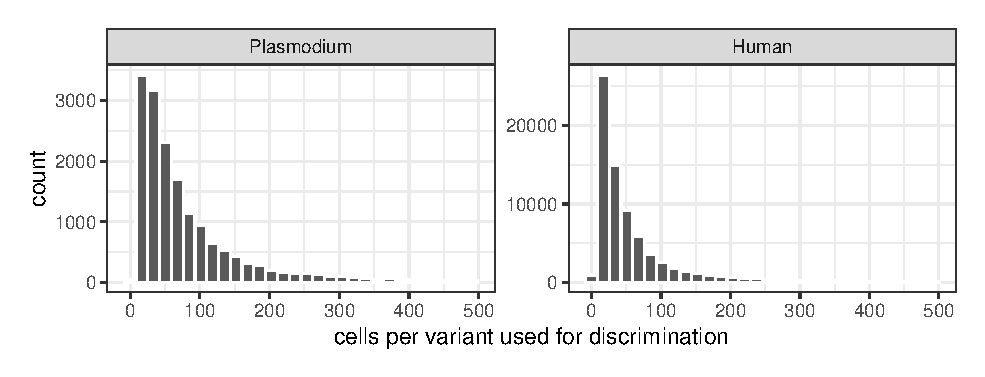
\includegraphics[width=\textwidth]{Cells_per_variant.eps}
\end{subfigure}
\begin{subfigure}[b]{\textwidth}
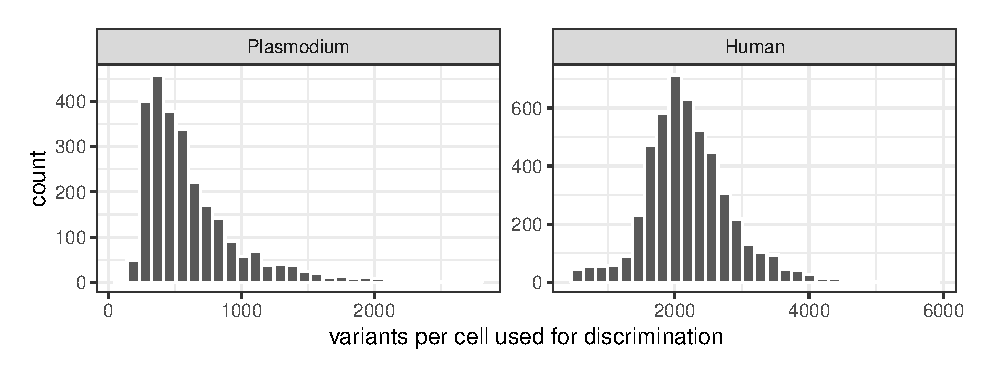
\includegraphics[width=\textwidth]{Variants_per_cell.eps}
\end{subfigure}
\end{centering}
\end{figure}

We wish to both determine which cells contain the same genotypes, but also what those genotypes are, and we achieve this with sparse mixture model clustering. \\

\textbf{Definitions}
\begin{itemize}
\item $K$: number of genotype clusters to be fixed at outset. Lower case $k$ will be used for indexing and referring to a specific cluster.
\item $C$: number of cells. Lower case $c$ will be used for indexing and referring to a specific cell. This actually refers to a barcode which generally comes from a single droplet but could correspond to multiple droplets. This barcode could have 0, 1, or more cells. It is important for some assumptions in this model that the majority of barcodes contain a single cell.
\item $L$: number of variant loci. Lower case $l$ will be used to index and refer to a specific loci. We will assume only biallelic variants. $L_c$ will be a list of loci with observed data in cell $c$.
\item $A$: Allele counts. $A_{l,c}$ is a vector of size 2 with the first number representing the number of reference alleles and the second value representing the number of alt alleles seen at locus $l$ in cell $c$.
\item $\phi_{k,l}$: mixture parameter for allele fractions of cluster $k$ at locus $l$. This is a real number representing the fraction of ref alleles in this cluster at this locus. We expect this to be near 1.0 (homozygous reference), 0.5 (heterozygous), or 0.0 (homozygous alt) but will be skewed from these values by noise, doublets, and ambient RNA.
\end{itemize} 

\noindent
\subsubsection{Model}

Weuse a maximum likelihood strategy by maximizing $p(data)$ under a given model. 
\begin{equation}
\argmax_{\phi} p(data, \phi)
\end{equation}
For each cell we marginalize across the clusters it could belong to and at each locus the reference allele count is modeled by a binomial with $n$ as the reference + alternative allele counts for that cell at that locus and $p$ as the mixture parameter for that cluster at that locus.
\begin{equation}
p(A,\phi) = \prod_{c \in C} \sum_{k \in K} \frac{1}{K} \prod_{l \in L_c}  \binom{A_{l,c,0} + A_{l,c,1}}{A_{l,c,0}} \phi_{k,l}^{A_{l,c,0}} (1-\phi_{k,l})^{A_{l,c,1}}
\end{equation}
Generally we minimize the negative log probability, which in this case is differentiable and thus susceptible to numerical optimization techniques such 
as gradient descent. It is worth noting here that the binomial probability of $0$ counts with $n=0$ is always $1$ for any $p$ and thus for a given cell $c$ we can ignore 
loci which have no observed counts of either allele. We solve this optimization problem with the machine learning package tensorflow with a custom loss function and 
the Adam optimizer which is a type of gradient descent using decaying momentum \cite{ADAM}. In practice 
the loss function that we actually use is the following 
\begin{equation}
loss = -log\bigg[\prod_{c \in C} \sum_{k \in K} \frac{1}{K} \prod_{l \in L_c} exp^{-\bigg(\frac{A_{l,c,0}}{A_{l,c,0}+A_{l,c,1}} - \phi_{k,l}\bigg)^2}\bigg]
\end{equation}
due primarily to not understanding how to use tensorflow probability distributions in which the parameters of the distribution are variable values. 
We have since found a solution to this but have not yet implemented it.
And treating this as a log probability we can calculate a pseudo-posterior cell assignments to clusters
\begin{equation}
p(c \in K_j) \approx \frac{\prod_{l \in L_c} exp^{-\bigg(\frac{A_{l,c,0}}{A_{l,c,0}+A_{l,c,1}} - \phi_{j,l}\bigg)^2}}{\sum_{k \in K} \prod_{l \in L_c} exp^{-\bigg(\frac{A_{l,c,0}}{A_{l,c,0}+A_{l,c,1}} - \phi_{k,l}\bigg)^2}}
\end{equation}

And the posteriors for cell $c$ being in cluster $j$ are as follows
\begin{equation}
p(c \in K_j) = \frac{\prod_{l \in L_c}  \binom{A_{l,c,0} + A_{l,c,1}}{A_{l,c,0}} \phi_{j,l}^{A_{l,c,0}}(1-\phi_{j,l})^{A_{l,c,1}}}{\sum_{k \in K} \prod_{l \in L_c}  \binom{A_{l,c,0} + A_{l,c,1}}{A_{l,c,0}} \phi_{k,l}^{A_{l,c,0}}(1-\phi_{k,l})^{A_{l,c,1}}}
\end{equation}

This method, as is the case with many clustering methods, may suffer from local minima in instances of poor initialization of the cluster centers $\phi$. To get around this, 
we run this method a number of times (generally 15) and take the minimum loss across these randomized iterations.


\subsection{Deterministic Annealing} 

\subsection{Doublet cell barcode detection}
One of the major aims of this work is to detect the barcodes which contain multiple cells with different genotypes. 
We are not, however, attempting to detect barcodes which contain multiple cells with the same genotype. We assume that 
the generation of doublet cell barcodes is a random poisson process and that the $\lambda$ of this poisson process is low enough that 
the chance of multiplets > 2 are exceedingly unlikely. We view this problem 
as a multi-urn problem in which we each locus is an urn containing either the allele counts of the best fitting cluster for this cell or the allele counts of
the combination of the top two clusters for this cell.

\textbf{Doublet model: Urn problem}
\noindent
\textbf{Definitions}
\begin{itemize}
\item $A_{k,l}$: Allele counts at locus $l$ for all cells in cluster $k$ according to the maximum probability cluster assignment from our clustering. This is a vector of size two with the ref and alt allele counts. 
\item $K_{c}$: Will be used to denote the list of clusters for cell $c$ ordered from the maximum posterior probability to the minimum. Thus $K_{c,0}$ is the cluster with the highest posterior probability for cell $c$. And for ease of notation we will denote $A_{K_{c,0 \cup 1},l}$ as the sum of the allele counts of those two clusters.
\end{itemize}
This can be computed directly.
\begin{equation}
p(c \in K_{c,0}) = \prod_{l \in L} \binom{A_{l,c,0} + A_{l,c,1}}{A_{l,c,0}} \frac{A_{K_{c,0},l,0}}{A_{K_{c,0},l,0} + A_{K_{c,0},l,1}}^{A_{l,c,0}} \bigg(1-\frac{A_{K_{c,0},l,0}}{A_{K_{c,0},l,0} + A_{K_{c,0},l,1}}\biggm)^{A_{l,c,1}}
\end{equation}
Beta binomial
\begin{equation}
p(c \in K_i) = \prod_{l \in L_c} \binom{A_{l,c,0} + A_{l,c,1}}{A_{l,c,0}} \frac{\beta (A_{l,c,0} + 1 + A_{i,l,0}, A_{l,c,1} + 1 + A_{i,l,1})}{\beta (1 + A_{i,l,0}, 1 + A_{i,l,1})}
\end{equation}

\begin{equation}
alpha_{l,i,j} = 1+ \frac{\frac{A_{i,l,0}}{A_{i,l,0}+A_{i,l,1}} +  \frac{A_{j,l,0}}{A_{j,l,0}+A_{j,l,1}}}{2}min(A_{i,l,0}+A_{i,l,1}, A_{j,l,0}+A_{j,l,1})
\end{equation}
\begin{equation}
beta_{l,i,j} = 1+ \frac{\frac{A_{i,l,1}}{A_{i,l,0}+A_{i,l,1}} +  \frac{A_{j,l,1}}{A_{j,l,0}+A_{j,l,1}}}{2}min(A_{i,l,0}+A_{i,l,1}, A_{j,l,0}+A_{j,l,1})
\end{equation}
\begin{equation}
p(c \in K_{i} \cup K_{j}) = \prod_{l \in L_c} \binom{A_{l,c,0} + A_{l,c,1}}{A_{l,c,0}} \frac{\beta (A_{l,c,0} + alpha_{l,i,j}, A_{l,c,1} + beta_{l,i,j})}{\beta (alpha_{l,i,j},  beta_{l,i,j})}
\end{equation}

\begin{equation}
p(doublet_c | c) = \frac{p(c \in K_{i} \cup K_{j})p(doublet)}{p(c \in K_{i} \cup K_{j})p(doublet) + p(c \in K_i)(1-p(doublet))}
\end{equation}

And the probability of the doublet case is 
\begin{equation}
p(c \in K_{c,0} \cup K_{c,1}) =  \prod_{l \in L} \binom{A_{l,c,0} + A_{l,c,1}}{A_{l,c,0}} 
\frac{A_{K_{c,0 \cup 1},l,0}}{A_{K_{c,0 \cup 1},l,0} + A_{K_{c,0 \cup 1},l,1}}^{A_{l,c,0}} \bigg(1-\frac{A_{K_{c,0 \cup 1},l,0}}{A_{K_{c,0 \cup 1},l,0} + A_{K_{c,0 \cup 1},l,1}}\biggm)^{A_{l,c,1}}
\end{equation}
And we can simply normalize these probabilities to sum to one for rough posteriors. We could also give the doublet vs singlet case a prior probability, but here we assume uniform chance. We then remove these doublets before moving on to the ambient RNA detection and cluster genotype inference.


\subsection{Ambient RNA detection and Cluster genotype inference}
One major goal of clustering scRNAseq by genotypes is calling the genotypes of each loci for each cluster.
But as previously discussed, there can be lysed cells in solution prior to cell partitioning which contribute a background noise to both genotypes and transcriptional profiles. 
This ambient RNA gives a fuzzy picture of the transcriptional profile and makes cluster genotypes which are in truth homozygous appear heterozygous. 
Luckily with genotype mixtures, we can use our prior knowledge of the ploidy of the mixed organisms along with our genotype cluster assignments to 
make a co-inference of both the genotypes and level of ambient RNA in the experiment.

\subsubsection{Mixture model of ambient RNA and cell RNA}

\noindent
\textbf{Definitions}
\begin{itemize}
\item $\rho$: mixture parameter representing the probability any given allele is arising from ambient RNA as opposed to from the cell associated with that barcode.
\item $P$: ploidy. We assume ploidy is limited to 1 or 2.
\item $A_l$: total allele expression at locus $l$. This is again a vector of length 2 denoting the reference and alternative allele counts.
\item $g$: used to denote the number of copies of the reference allele. So the expected reference allele rate without ambient RNA is $\frac{g}{P}$ and $g$ is an integer value $\in [0..P]$. And it is worth noting that this one number is sufficient to denote the genotypes for ploidy 1 and 2.
\item $p(true)$: probability variant is a true positive. 
\end{itemize}

Once again we solve this with a maximum likelihood approach.
\begin{equation}
\argmax_{\rho} p(data, \phi)
\end{equation}
And the model treats each locus in each cluster as coming from one of three genotypes for diploid (0/0, 0/1, 1/1, here denoted by g=0,1, or 2) and two genotypes from haploid (0, 1). We 
treat each cluster as independent and each locus as independent. Then we marginalize across the possible genotypes.  
And so we model the allele counts in this cluster as having come from 
a mixture of ambient RNA and from this cells in this cluster. And then we model the observed allele fractions as being drawn from a binomial distribution 
with a probability which was skewed away from $p=\frac{g}{P}$ by the level of ambient RNA. And we believe that the ambient RNA is drawn from 
an average of all of the reads in the experiment. As such, the expected allele fraction coming from the soup is $\frac{A_{l,0}}{A_{l,0} + A_{l,1}}$. 
Thus, the probability of the binomial of the mixture of cell data is the following.
\begin{equation}
p_{tp} = (1-\rho)\frac{g}{P} + \rho \frac{A_{l,0}}{A_{l,0}+A_{l,1}}
\end{equation}
\begin{equation}
p_{fp} = \frac{A_{l,0}}{A_{l,0}+A_{l,1}}
\end{equation}



Now we use that binomial probability in the full likelihood.
\begin{equation}
\begin{split}
p(data | \rho) = \prod_{l \in L} \bigg[ & p(true) \prod_{k \in K} \sum_{g = 0}^P \frac{1}{P} \binom{A_{k,l,0} + A_{k,l,1}}{A_{k,l,0}} p_{tp}^{A_{k,l,0}} (1-p_{tp})^{A_{k,l,1}} \\
 & + (1-p(true))\prod_{k \in K}\binom{A_{k,l,0} + A_{k,l,1}}{A_{k,l,0}}p_{fp}^{A_{k,l,0}} (1-p_{fp})^{A_{k,l,1}}  \bigg]
\end{split}
\end{equation}

\subsubsection{Inference}
And we solve this in a maximum likelihood fashion using STAN which is a domain specific language for probabilistic models.

And the posteriors for genotypes for each locus for each cluster can easily be computed by normalizing the binomial probabilities over all possible genotypes.


%********************************** %Second Section  *************************************
\section{Results}
In order to analyze our results we must first create a ground truth dataset to compare it to. We have the whole genome sequencing data for each 
of these strains and individuals, so we can use demuxlet \cite{demuxlet} to assign cells to these known genotypes as well as call doublets. In doing this 
we ran into several problems. First, we ran demuxlet on the malaria data which is a mixture of six strains of \textit{Plasmodium falciparum} and it claimed 
that every cell was from the 3D7 strain. As we found this to be unlikely given the experimental setup which aimed to get an even mixture of strains we looked into 
things further. We found that the indel calls on the WGS data were poor due to the extremely A/T rich nature of the \textit{Plasmodium} genome. So 
we then removed the indels and reran demuxlet. It then showed all cells as 3D7 except for some doublets of 3D7 and other strains. It should be noted here 
that the reference used for mapping the WGS data was created from the 3D7 strain. So we suspected that reference bias might be a serious issue. We then remapped all 
of the WGS data to a reference created from a strain that this experiment did not contain. We then got a good mixture of cell assignments, but the doublet detection rate 
was an order of magnitude higher than the expected doublet rate given the number of input cells. On further analysis we have decided that this overestimation of 
doublets is due to the ambient RNA. So for our analysis we will compare to the demuxlet best call ignoring whether the cell was also called a doublet as well as to the demuxlet 
calls ignoring demuxlet called doublets.

\subsection{Benchmarking: Synthetic human cell mixture vs real human cell mixture}

\subsubsection{Validation and comparison to other methods}

Samples have been ordered such that the primary numbers show up on the diagonal.
\begin{table}[h!]
\begin{center}
\caption{Clustering concordance of human scRNAseq replicate 1 with Demuxlet}
\label{table:H1clust}
\begin{tabular}{ | c | c | c | c | c | c | c | } 
\hline
\multicolumn{2}{|c|}{} & \multicolumn{5}{c|}{Demuxlet best sample} \\
\cline{3-7}
\multicolumn{2}{|c|}{} & euts & babz & nufh & oaqd & ieki \\
\hline
\multirow{6}{4em}{Cluster} & 0 & 1110 & 1 & 0 & 9 & 0 \\
					 \cline{2-7}
                                           & 1 & 7 &  800 & 1 & 5  & 6  \\
                                           \cline{2-7}
                                           & 2 & 4 & 5 & 691 & 9 & 3 \\
                                           \cline{2-7}
                                           & 3 & 7 & 0 & 2 & 1640 & 7 \\
                                           \cline{2-7}
                                           & 4 & 3 & 2 & 1 & 0 & 612 \\
                                           \hline
\end{tabular}
\end{center}
\end{table}

\begin{table}[h!]
\begin{center}
\caption{Clustering concordance of human scRNAseq replicate 2 with Demuxlet}
\label{table:H2clust}
\begin{tabular}{ | c | c | c | c | c | c | c | } 
\hline
\multicolumn{2}{|c|}{} & \multicolumn{5}{c|}{Demuxlet best sample} \\
\cline{3-7}
\multicolumn{2}{|c|}{} & ieki & babz & eutz & oaqd & nufh \\
\hline
\multirow{6}{4em}{Cluster} & 0 & 628 & 0 & 5 & 1 & 0 \\
					 \cline{2-7}
                                           & 1 & 2 & 794 & 8 & 3 & 1 \\
                                           \cline{2-7}
                                           & 2 & 2 & 3 & 1133 & 3 & 0 \\
                                           \cline{2-7}
                                           & 3 & 1 & 4  & 3 & 1523 & 2 \\
                                           \cline{2-7}
                                           & 4 & 7 & 2 & 5 & 9 & 693 \\
                                           \hline
\end{tabular}
\end{center}
\end{table}

\begin{table}[h!]
\begin{center}
\caption{Clustering concordance of human scRNAseq replicate 3 with Demuxlet}
\label{table:H3clust}
\begin{tabular}{ | c | c | c | c | c | c | c | } 
\hline
\multicolumn{2}{|c|}{} & \multicolumn{5}{c|}{Demuxlet best sample} \\
\cline{3-7}
\multicolumn{2}{|c|}{} & nufh & eutz & babz & oaqd & ieki \\
\hline
\multirow{6}{4em}{Cluster} & 0 & 732 & 0 & 3 & 14 & 4 \\
					 \cline{2-7}
                                           & 1 & 2 & 1241 & 7 & 5 & 1 \\
                                           \cline{2-7}
                                           & 2 & 3 & 2 & 805 & 4 & 4 \\
                                           \cline{2-7}
                                           & 3 & 0 & 4  & 2 & 1655 & 4 \\
                                           \cline{2-7}
                                           & 4 & 1 & 0 & 0 & 1 & 650 \\
                                           \hline
\end{tabular}
\end{center}
\end{table}

We currently do not have sc split run on these samples as the variant calling step is very computationally expensive in the way they suggest. We wish to have this comparison 
by the viva.

Giving adjusted rand indexes of $0.96$, $0.97$, and $0.97$ respectively. If we remove the demuxlet called doublets, the concordance is perfect on all three replicates.

The ambient RNA estimation for these samples is $19.4\%$, $18.8\%$, and $19.2\%$ respectively which are currently unvalidated as are the inferred genotype calls.

The doublet analysis code was written on a previous clustering and variant calling strategy which output different formats and needs reworking to get results. We wish 
to complete this analysis in time for the viva.

\subsection{Maternal-Fetal data}



\subsection{Plasmodium}
Samples have been ordered such that the primary numbers show up on the diagonal of the confusion matrix.
\begin{table}[h!]
\begin{center}
\caption{Clustering concordance of malaria scRNAseq dataset with Demuxlet}
\label{table:malariaclust}
\begin{tabular}{ | c | c | c | c | c | c | c | c |} 
\hline
\multicolumn{2}{|c|}{} & \multicolumn{6}{c|}{Demuxlet best strain} \\
\cline{3-8}
\multicolumn{2}{|c|}{} & 3D7 & GB4 & 7G8 & 11.02 & 15.04 & 28.04 \\
\hline
\multirow{6}{4em}{Cluster} & 0 & 1132 & 0 & 0 & 1 & 1 & 0 \\
					 \cline{2-8}
                                           & 1 & 1 & 414 & 0 & 0 & 0 & 0 \\
                                           \cline{2-8}
                                           & 2 & 0 & 0 & 274 & 0 & 0 & 0 \\
                                           \cline{2-8}
                                           & 3 & 0 & 0 & 1 & 242 & 0 & 0 \\
                                           \cline{2-8}
                                           & 4 & 0 & 0 & 0 & 0 & 219 & 0 \\
                                           \cline{2-8}
                                           & 5 & 1 & 0 & 0 & 0 & 0 & 321 \\
                                           \hline
\end{tabular}
\end{center}
\end{table}

Which gives an adjusted rand index of 0.995. Excluding cells called by demuxlet as doublets ($23.7\%$) there is perfect concordance. 

Sc split \cite{sc_split} was a tool recently released with this same goal in mind and we have run it on this dataset and here show the comparison 
of that tool to demuxlet. This is already removing cells called doublets by sc split ($13\%$) but not removing cells called doublets by demuxlet.

\begin{table}[h!]
\begin{center}
\caption{sc split concordance of malaria scRNAseq dataset with Demuxlet}
\label{table:scsplitmalaria}
\begin{tabular}{ | c | c | c | c | c | c | c | c |} 
\hline
\multicolumn{2}{|c|}{} & \multicolumn{6}{c|}{Demuxlet best strain} \\
\cline{3-8}
\multicolumn{2}{|c|}{} & 7G8 & 3D7 & GB4 & 11.02 & 15.04 & 28.04 \\
\hline
\multirow{6}{4em}{Cluster} & 0 & 222 & 1 & 1 & 3 & 8 & 2 \\
					 \cline{2-8}
                                           & 1 & 0 & 559 &  0 & 1 & 0 & 1 \\
                                           \cline{2-8}
                                           & 2 & 0 & 1 & 386 & 1 & 0 & 1 \\
                                           \cline{2-8}
                                           & 3 & 1 & 2 & 12 & 224 & 79 & 5 \\
                                          \cline{2-8}
                                           & 4 & 0 & 566 &1  & 1 & 0 & 2 \\
                                           \cline{2-8}
                                           & 5 & 52 & 1 & 7 & 11 & 111 & 7 \\
                                           \hline
\end{tabular}
\end{center}
\end{table}

This clustering seen in table \ref{table:scsplitmalaria} gives an adjusted rand index of $0.62$ splitting 3D7 into two clusters and combining some others and also identifying nearly all of the $28.04$ strain as doublets.


\subsection{Twenty one individual mixture demonstration}
\subsubsection{Contamination revealed}

\section{Discussion}
We have presented a collection of novel methods for use in mixed sample single cell RNAseq datasets and have shown that they significantly out perform current competing methods 
for clustering cells by genotype. For doublet detection we have good reason to believe that our approach will yield more accurate doublet calls than either demuxlet or sc split in the presence 
of significant ambient RNA. And we also have good reason to believe that our genotype calls will be of higher quality. These last two things we hope to have more analysis on by the time 
of the first year viva.


%********************************** % Third Section  *************************************

